\section{Vision for Implementation}
\label{sec:implementation}

As the prototyping of TrustFA is still in progress, we envision its
implementation on Freescale i.MX53 Quick Start Board (QSB) \cite{imx53qsb}. The
board is equipped with a Cortex-A8 single core with processing speeds up to 1.2
GHz and 1GB DDR memory.  Although our vision requires specific registers on i.MX53 QSB, registers
achieving the same functionalities are available on other development boards,
e.g., Freescale i.MX6 SABRE Lite \cite{imx6sabrelite}.

\noindent
{\bf Secure Boot~}
The execution of TrustZone's secure world starts with the secure boot provided
by the on-chip boot ROM. The i.MX53 processor provides this capability with the
High Assurance Boot (HAB) component.  The HAB uses digital
signatures to authenticate the TrustZone secure world bootloader, which executes
immediately after the on-chip boot ROM. The verified bootloader can then verify
other secure kernel. HAB authentication is based on public key cryptography
using the RSA algorithm in which image data is signed offline using a series of
private keys. The resulting signed image data is then verified on i.MX53
processor using the corresponding public keys. Freescale Code Signing Tools HAB
does this by computing a cryptographic hash of the Super Root Key (SRK) table
and comparing the result with a pre-computed hash that is provisioned in
One-time programmable (OTP) fuses. Attacker with unsigned image would not be
able to boot the device.

\noindent
{\bf Secure Memory~}
We achieve memory isolation using the Multi-Master Multi-Memory Interface
(M4IF), which supports two chunks of physically continuous secure memory. The
secure memory can only be configured when the CPU is in TrustZone secure mode.
Even after being compromised, the normal world legacy OS is not allowed to
access TrustFA Agent and secure kernel. M4IF\_WMSA and M4IF\_WMEA registers
define the start and end address of the secure memory chunks respectively.
M4IF\_WMIS registers enable the protection of each secure memory chunk. The DDR
memory range of i.MX53 is 0x70000000-0xEFFFFFFF (1GB) and we assign
0xc0000000-0xEFFFFFFF (386MB) as secure world memory.

\noindent
{\bf Secure Peripheral~}
We use Central Security Unit (CSU) registers to configure the control policies
between bus masters and bus slaves. This will allow us to separate the
peripherals into distinct security worlds and prevent the normal world OS from
gaining access to secure world peripherals, e.g., camera, accelerometer and
touch screen. Besides, normal world peripherals are not able to access secure
world memory via DMA. TZIC\_INTSEC registers in TrustZone Aware Interrupt
Controller (TZIC) specify whether each peripherals are in secure world or normal
world.

\noindent
{\bf Preliminary Evaluation~}
The development of TrustFA is still in progress. We have successfully booted a
simple bare-metal program in TrustZone secure world. The secure program then
boots the Linux 2.6.38 in normal world. We have configured secure memory so that
normal world Linux is not able to read/write data in secure world.

Figure \ref{fig:syscall} shows the performance overhead of TrustZone world
switch.  We implement a new system call which triggers a null SMC call in secure
world (including the context switch between secure and normal world). We compare
its performance overhead with null, getpid and fork system calls. Each system
call is called 10 times and we measure the overhead of 10 calls together. The
total overhead of 10 null system call is $13.2\mu s$. As in Figure
\ref{fig:syscall}, SMC system call is 7.8 times of null system call.  Compared
to fork, which is 242 times of null system call, the performance overhead of SMC
is trivial. Actually, the data cache and instruction cache are disabled in
secure world during the evaluation. The overhead of SMC would become
less if we enable the cache in the final prototype of TrustFA.

\begin{figure}[htb]
	\centering
	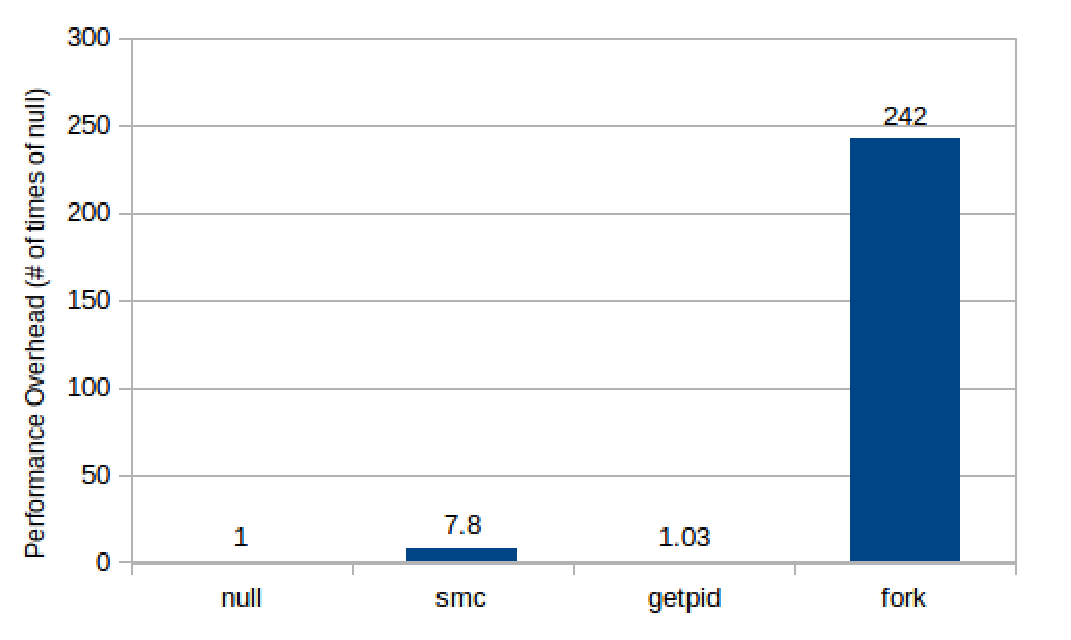
\includegraphics[width=1.0\columnwidth]{figures/syscall.eps}
	\caption{Performance Overhead Comparison of System Calls}
	\label{fig:syscall}
\end{figure}
